\documentclass{beamer}
\usetheme{Goettingen}
\usecolortheme{sidebartab}

\title{Data Augmentation using GPT-2}
\author{Masaoud Haidar}
\subtitle{Statistics 98}
\institute{Harvard University}

\date{May 2022}

\begin{document}

\begin{frame}
    \titlepage
\end{frame}

\begin{frame}{Outline}
    \tableofcontents
\end{frame}

% Introducing GPT-2

% Text Data Augmentation
%% Imbalanced data + random sampling

% Research Question

% Literature Review

% Maybe Reasearch Question and Literature Review together and then add preliminary results at the end?

% Research Setup

\section{Background}
\begin{frame}
\frametitle{Imbalanced Data}

\begin{itemize}
\item Imbalanced data can result in biased models. One solution to this is to over-sample from minority data points. Simple Bootstrapping can lead to over-fitting, so we want to create new synthetic data. 
\end{itemize}

\end{frame}

\begin{frame}
\frametitle{Text Data Augmentation Methods}

\begin{itemize}
\item \textbf{EDA: Easy Data Augmentation}: 

Presented by Wei and Zou [2019]. Combines 4 methods:

\begin{enumerate}
    \item Synonym Replacement
    \item Random Insertion
    \item Random Swap
    \item Random Deletion
\end{enumerate}

Improves CNNs and RNNs. Works best on small datasets. On specific tasks, training with 50\% of data with EDA performs as well as training with all the data. 

\textbf{}

\item<2-> \textbf{GPT-2}

Presented by Radford et al. [2018] and [2019]. Can be used to generate new text data. Shown to improve F1 score on some tasks. Might not preserve the label When conditioned to generate data from multiple classes.

\end{itemize}

\end{frame}

\section{Inside GPT-2}

\begin{frame}{GPT-2 Structure}

\begin{columns}
\begin{column}{0.5\textwidth}
  \begin{itemize}

    \item<1-> Generative Pre-trained Transformer 2. Pre-trained on a large amount of data, and can be tuned for specific tasks. 
    
    \item<2-> Uses multiple layers of decoder-only transformers that use the self attention mechanism to transform the data. The output of the last layer is passed to a FFNN to predict the next word. 
\end{itemize}
\end{column}
\begin{column}{0.5\textwidth}  %%<--- here
    \begin{center}
         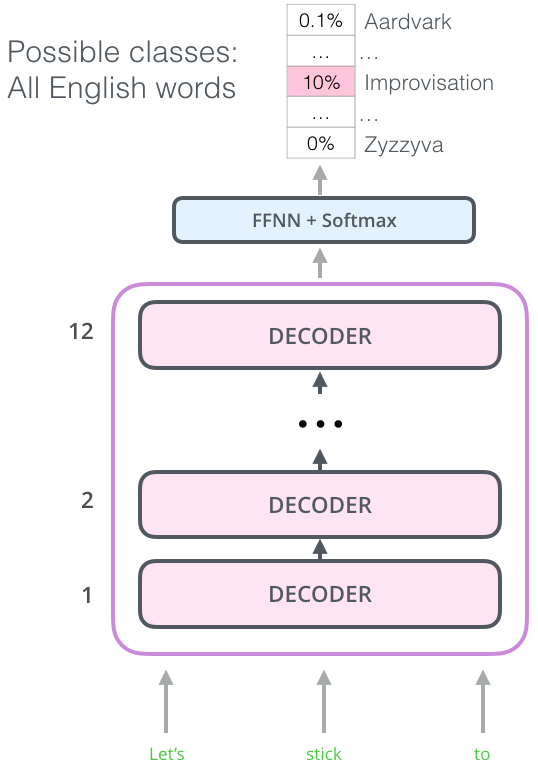
\includegraphics[width=1\textwidth]{gpt2.png}
     \end{center}
\end{column}
\end{columns}



\end{frame}

\section{Research Question}
\begin{frame}{Research Question}

\begin{itemize}
\item \textit{How does Data Augmentation using GPT-2 affect the distribution of the data? And how does it compare with EDA when used with word-based models or context-based models?} 
\end{itemize}

\end{frame}



\section{Experimental Setup}
\begin{frame}{Experimental Setup}

\begin{itemize}
\item<1-> Create 5 main Training Datasets:

\textbf{}
\begin{enumerate}[(A)]
    \item<1-> Main training set of Amazon Reviews. 80:20 rate. 
    
    \textbf{}
    \item<2-> Artificially Imbalanced training set. 95:5 rate
    
    \textbf{}
    \item<3-> Augment (B) using GPT-2 to 80:20 rate
    
    \textbf{}
    \item<4-> Augment (B) using GPT-2 to 90:10 rate
    
    \textbf{}
    \item<5-> Augment (B) using EDA to 80:20 rate.
\end{enumerate}

\textbf{}

\item<6-> We use Distilled GPT-2 for (C) and (D). \\ We use EDA with $\alpha = 0.1$ for (E)

\end{itemize}
\end{frame}

\begin{frame}{Experimental Setup}
\begin{itemize}

\item<1-> Record the following:
\begin{enumerate}[(1)]
    
    \item<1-> \textbf{Word-based Model Performance:} Train TF-IDF plus Logistical Regression classifier. Record the accuracy and F1 scores. 
    
    \textbf{}
    
    \item<2-> \textbf{Context-based Model Performance:} Train a BERT Classifier. Record the accuracy and F1 scores. 
    
    We use tiny-bert with only two layers of encoder transformers.
    
    \textbf{}
    
    \item<3-> \textbf{Distribution of the Data:} We compare the distribution of the data in (A), (D), and (E).
    
    \textbf{}
    
    \item<4-> \textbf{Preserving Labels:} Which is better at preserving labels, (D) or (E)?
\end{enumerate}

\end{itemize}
\end{frame}

\section{Results}
\begin{frame}{Word-Based Model Performance}

\begin{center}
\begin{tabular}{||c c c||} 
 \hline
 Model & Accuracy & F1 Score \\ [0.5ex] 
 \hline\hline
 A. Original & 0.8799 & 0.662  \\ 
 \hline
 B. Imbalanced & 0.821 &  0.246 \\
 \hline
 C. GPT2 & 0.8366 &  0.4209 \\
 \hline
 E. EDA &  0.8189 & 0.2715 \\
 [1ex] 
 \hline
\end{tabular}
\end{center}

\end{frame}

\begin{frame}{Context-Based Model Performance}

\begin{center}
\begin{tabular}{||c c c||} 
 \hline
 Model & Accuracy & F1 Score \\ [0.5ex] 
 \hline\hline
 A. Original & 0.8886 & 0.7002  \\ 
 \hline
 B. Imbalanced & 0.8443 & 0.4198 \\
 \hline
 C. GPT2 & 0.8403 &  0.4289 \\
 \hline
 E. EDA &  0.7931 & 0.0038 \\
 [1ex] 
 \hline
\end{tabular}
\end{center}

\end{frame}

\begin{frame}{Distribution of the Data}
\begin{itemize}
    \item Train a Base BERT (the original large model) on (A). Record the outputs of the last layer of the model (before classification). Make TSNE plot of 500 samples from each group.
\end{itemize}

\begin{center}
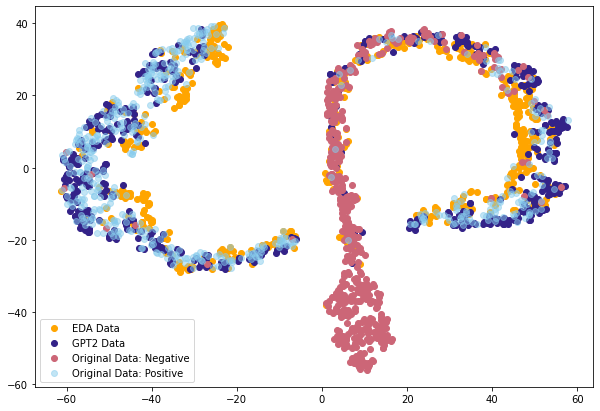
\includegraphics[width=0.8\textwidth]{tsne.png}
\end{center}
\end{frame}

\begin{frame}{Preserving Labels}
\begin{itemize}
\item<1-> Editing too much in a data point can change its meaning, and thus change its label. We want to measure that.

\textbf{}

\item<2-> Train a Base BERT (the original large model) on (A). Record the accuracy on the generated samples.

\textbf{}

\item<3-> The model achieves 90.9\% accuracy on the positive data from its training set. \\
Achieves 76.32\% accuracy on the GPT-2 data. \\
Achieves 64.16\% accuracy on the EDA data.

\end{itemize}
\end{frame}

\section{Conclusions}

\begin{frame}{Conclusions}
\begin{itemize}
\item<1-> Models trained on GPT2-Augmented Datasets do better than EDA-Augmented datasets in all tested settings. GPT2 is also better at preserving the minority labels.

\textbf{}

\item<2-> On TF-IDF with logistical regression, GPT-2 improves the F1 score by 18 points. 

\textbf{}

\item<3-> With tiny-bert, it only improves F1 score by 0.9\%. Might be because BERT was already not very prone to Imbalanced Data. 

\textbf{}

\item<4-> Models trained on (C) and (E) don't come close to the models trained on original data. There is a lot of work to be done on imbalanced data.


\end{itemize}
\end{frame}

\end{document}
